\documentclass[10pt]{standalone}
\usepackage{tikz}
\usetikzlibrary{shapes.geometric,fit}
\begin{document}
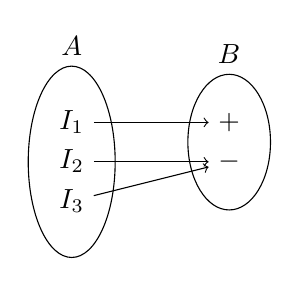
\begin{tikzpicture}
    \foreach[count=\i] \lseti/\lsetmi in {A/{$I_1$,$I_2$,$I_3$},B/{$+$,$-$}} {
        \begin{scope}[local bounding box=\lseti, x=2cm, y=0.5cm]
        \foreach[count=\j] \lj in \lsetmi {
            \node[minimum width=1em,anchor=base,text height=1.4ex,text
            depth=0.25ex] (n-\j-\lseti) 
            at (\i,-\j) {\lj};
        }
        \end{scope}
        \node[ellipse, draw, fit=(\lseti), 
        label={[name=l-\lseti]above:$\lseti$}] {};
    }
    \draw[->] (n-1-A) -- (n-1-B);
    \draw[->] (n-2-A) -- (n-2-B);
    \draw[->] (n-3-A) -- (n-2-B);
    %\draw[->] (l-A) -- node[above]{$f$}(l-B);
\end{tikzpicture}
\end{document}